\section{A feature model to characterize software traceability}\label{sec:fm}
%\ugh{This is paraphrase from SDI speech-to-text}
This section presents our conceptualization of traceability by means of a feature model describing the traceability features and dimensions found in the analysis of the literature conducted in the previous section. Our feature model groups them by similarity and provides additional descriptions on the most important aspects of each one, \textit{e.g.}, different existing alternative implementation of the same feature and/or the most/the least studied ones in each group.  

%we present a classification that cover components needed for traceability, based on a set of common characteristics found in selected studies from previous section. Considering the lack of a consolidated terminology in the literature, we have extracted the characteristics and grouped them by similarity. Next, a generic nomenclature was assigned for each group, so that similar characteristics in a group are represented in an unified way. 

Next subsections provide some background on feature modeling and then zoom in each of the three main dimensions of traceability: trace representation, trace identification, and trace management. These dimensions are depicted in \Fig{fig:fm:definition}, \Fig{fig:fm:identification}, and \Fig{fig:fm:management}, respectively. %The feature model was created focusing on the identification of the prominent or distinctive features, i.e., attributes of a system that directly affect end-users’ decisions. 

%Based on the analysis of the papers selected in the previous section, we propose a feature model for software traceability. 
%Our first finding is that the knowledge area of software traceability breaks down into three sub-areas. 
%For each of them, together with a more detailed explanation, we will present a feature model that summarizes the broad set of dimensions that must be considered when describing traceability proposals. 

%The first sub-area targets concerns directly related to trace definition and representation. \Sect{sec:fm:def} relates the associated techniques and distinguishes what kind of languages are used to represent traces and how expressive they are. E.g., is it possible to define types of traces? And use them to link clusters of artefacts (or just individual elements)? Can we express the confidence we have in those traces?  
%In the second sub-area, the means of identifying and recording traces are under scrutiny and differentiates configurations depending if traces need to be manually created or if they can be derived from existing information. If so, what methods can be used for such derivation? These are some of the topics related to trace identification that we would like to disentangle in our feature model in \Sect{sec:fm:identification}.
%Finally, the third sub-area distinguishes the techniques implemented to assist the storage and maintenance of quality traces. 

\subsection{Introduction to feature modelling}
A feature model leverages features as the abstraction mechanism to reason about product variability. It is a hierarchically arranged set of features, where relationships between a parent feature and its child features may be categorized as: \textit{and} – all sub-features must be selected, \textit{alternative} - only one subfeature can be selected, \textit{inclusive or} – one or more can be selected, \textit{mandatory} - features that are required, and \textit{optional} - features that are optional~\cite{kang1998-FeatureModel}.  Each feature represents an increment in product functionality. 

Feature modeling is a technique that has been intensively used for documenting the points of variability in a software product line, how the points of variability constraint one another, and what constitutes a complete configuration of the system. 
%This seminal work from Kang \textit{et al.} has been cited thousand times. To complement feature-modeling tooling, researchers contributed hundreds of feature-model analyses, refactorings and management techniques, as well as automated synthesis techniques. Feature modeling is supported by major product-line engineering tools~\cite{nesic2019-principles-of-FM}. 
But beyond product lines, feature model are also more and more used to shed light on complex domains by representing the core concerns and variation points in a complex ecosystems (\textit{e.g.}, \cite{DBLP:journals/sosym/BruneliereBCW19}), as we do in this paper.

%It can capture different types of variability, ranging from requirements variability to implementation variability. It can also allow for automated generation and verification of complex systems~\cite{metzger2007-feature-model-check}. 


\subsection{Trace definition and representation}
\label{sec:fm:def}
\begin{figure*}[h]
	\centering
	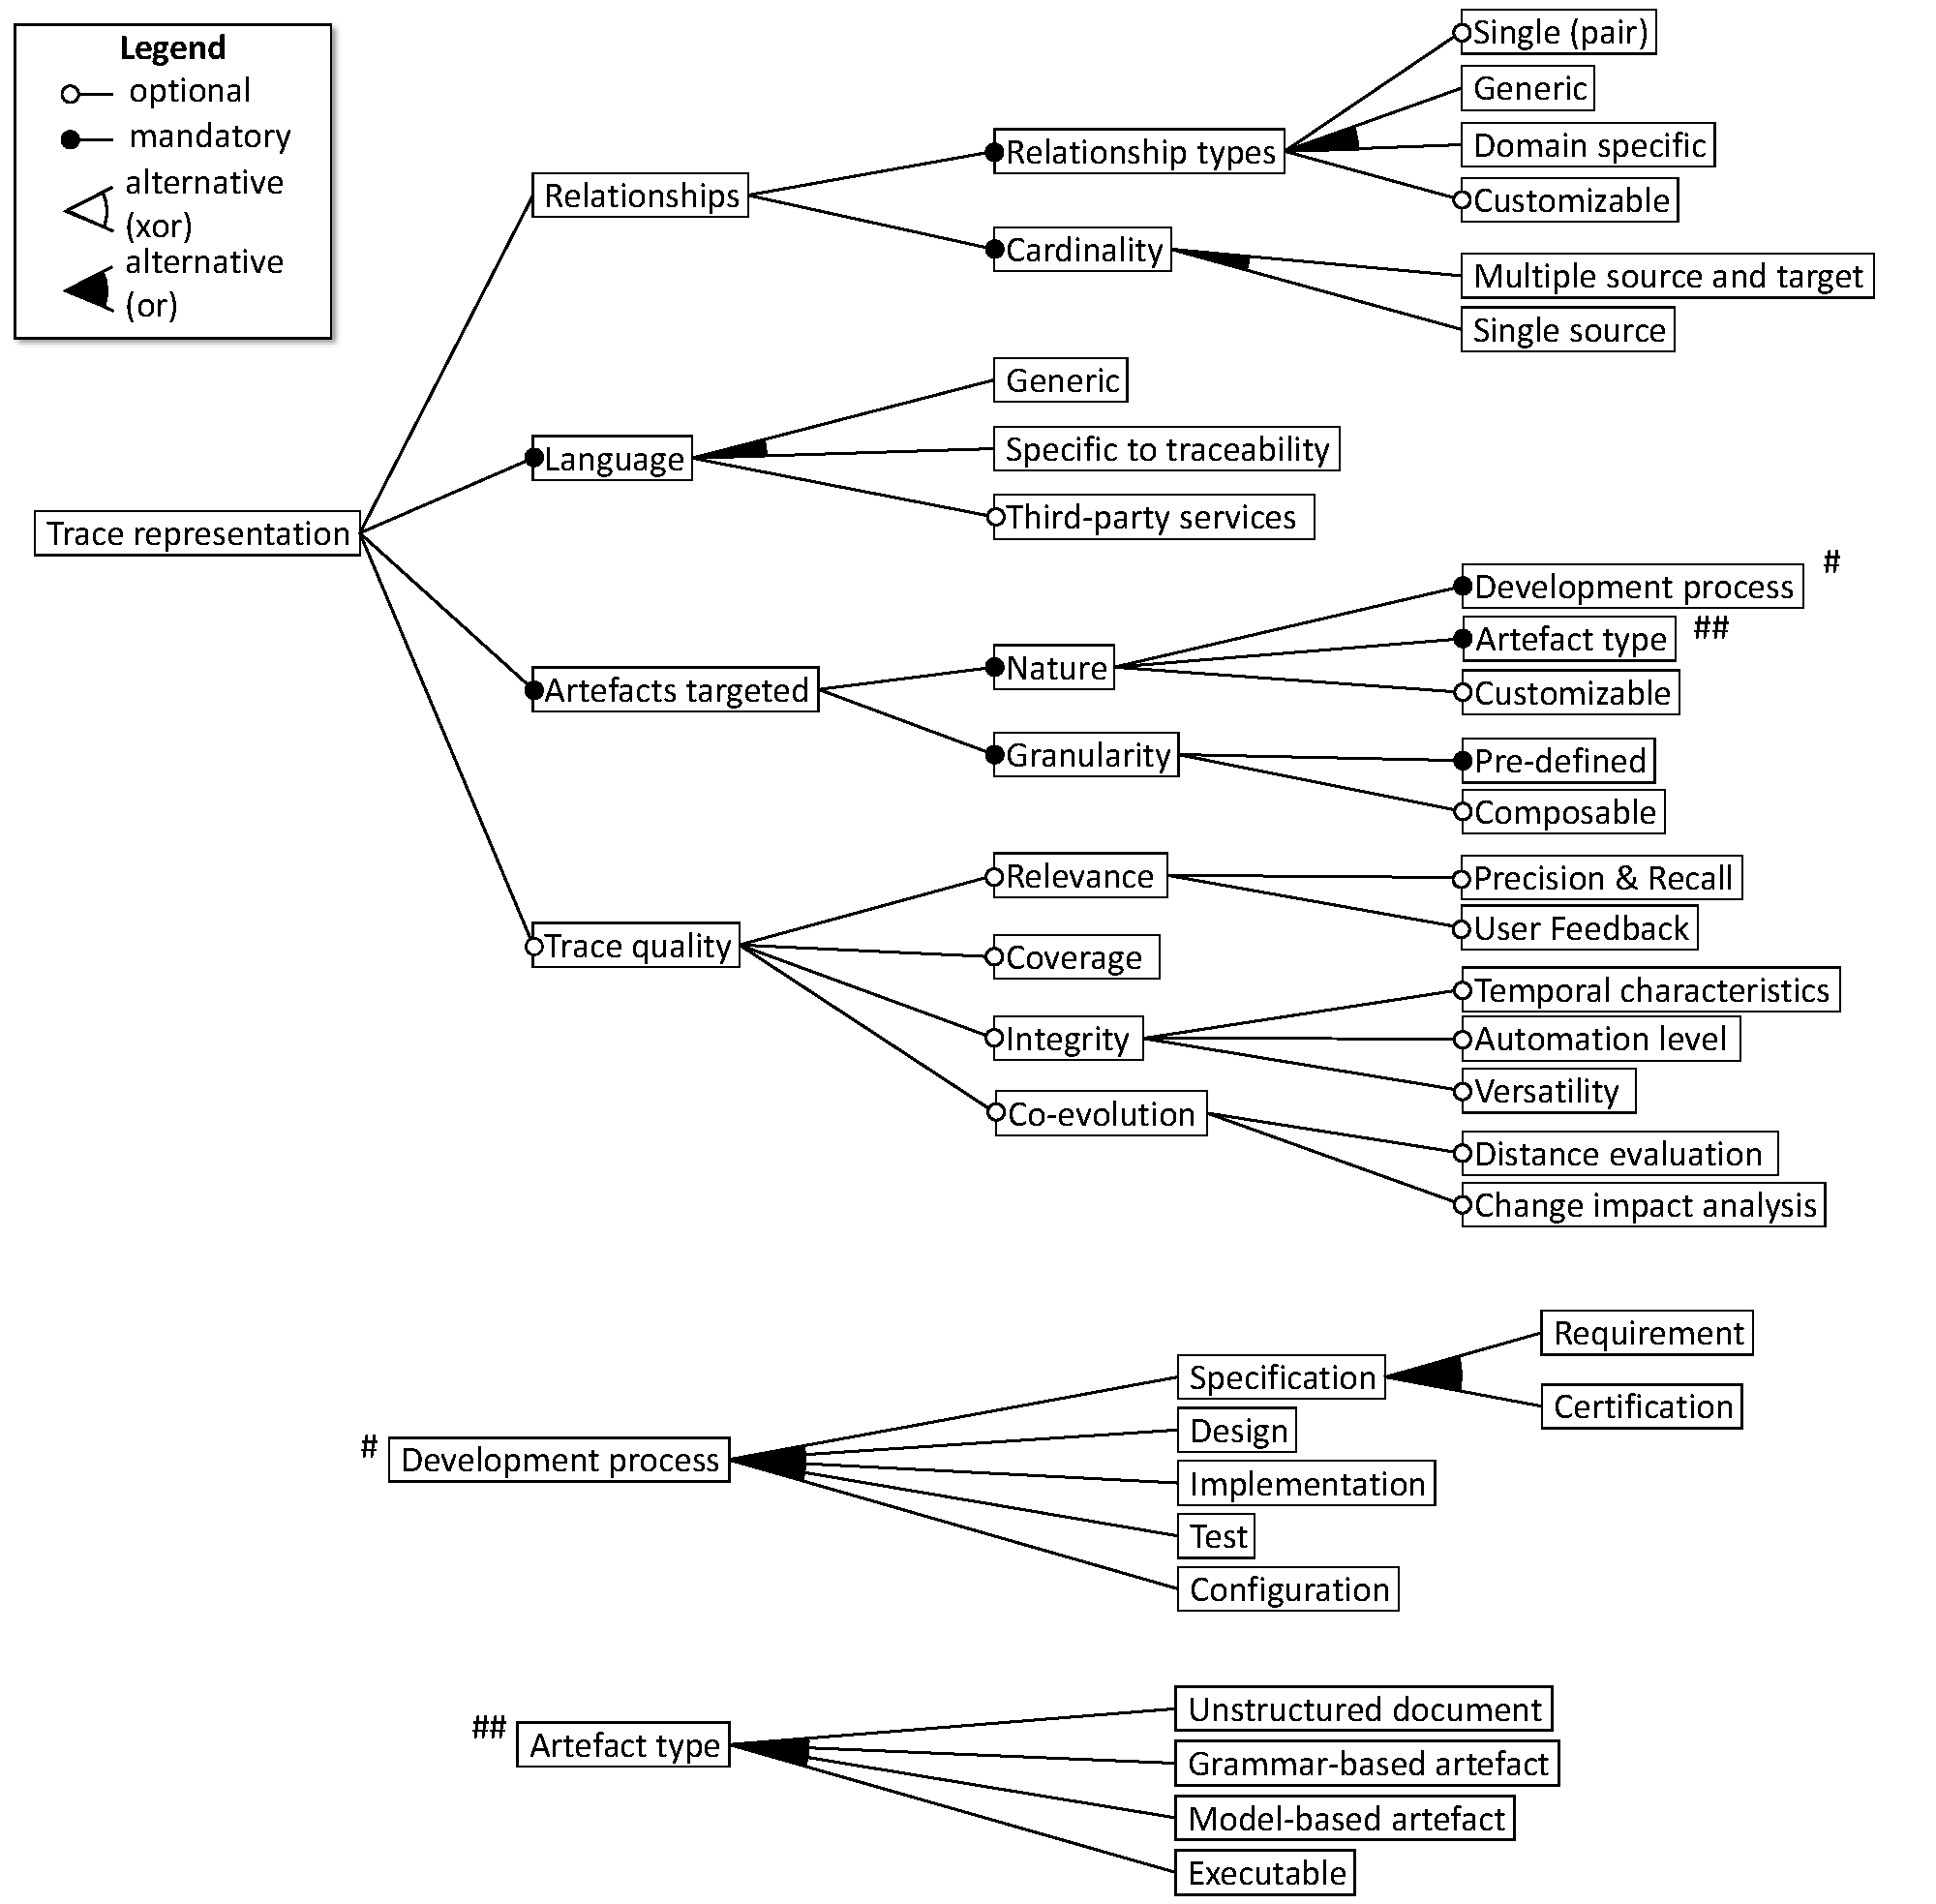
\includegraphics[width=.8\linewidth]{images/fm-definition}
	\caption{Features related to the representation of a trace.}
	\label{fig:fm:definition}
\end{figure*}

%As discussed in the terminology section, there is no common representation or standard for traceability. Instead, we find a plethora of applications of traceability in specific domains such as program understanding, with approaches facilitating the localisation of features~\cite{seiler2019-comparing-trac-through-IR-Commits-Logs} and bugs~\cite{ko2008-whyline-debugging}. Traceability eases software decomposition into relevant partitions~\cite{laghouaouta2017-model-composition-tracaebility} or slices~\cite{nejat2012-traceability-sysml-safety-certification}, it eases software reuse ~\cite{tinnes2019-improving-art-reuse-with-traceability} and provides support for the general explainability of the software process and product~\cite{wohlrab2020-traceability-organization-process-culture}. 
%Traces are used to help gath%er evidences for certification. 

All approaches must discuss their representation of trace artefacts even if they can differ already based on the type of traces they consider and their foreseen application. Representations are so diverse that our survey selected more than 80 papers mentioning their own distinct definitions with 20 metamodels effectively depicted in those papers.
Some researchers present generic graph-based representations ~\cite{schwarz2010-graph-based-traceability,grammel2012-model-matching-for-traceability-in-MDE} while others focus on representations much more specific to a concrete application like this metamodel for %  the verification and validation of software artefacts~\cite{Dubois_2010,vonknethen2002-change-oriented-req-traceability-evolution-of-embedded-systems} and traceability artefacts~\cite{rempl2014-conformance-of-traceability-to-guidelines} ; others target the maintenance of software systems with representations for 
change impact analysis~\cite{goknil2014-change-impact-analysis-for-requirement-metamodel} or multi-model consistency~\cite{Szabo_2013}.
%\eb{So many perspectives shall provide enough details for a standard, or at least a common understanding (cf our metamodel?).}

\Fig{fig:fm:definition} shows the hierarchy of features related to the definition and the representation of trace artefacts. A peculiar focus is put on the typing of the traces relationships. Typing relationships is important to add semantics to the trace so that the engineer can know not only what are the linked artefacts but also why they are linked. As such, it facilitates the  application of traceability solutions to specific domains. We also detail the genericity of the language, the artefacts covered by the traceability proposal and the possibility to annotate traces with quality properties.

We would like to remark the contribution of model-based approaches for traceability in this subsection. The use of MDE tooling such as ATL~\cite{Santiago_2013,Jim_nez_2013}, or the Eclipse Modeling Framework (EMF) allows the automated generation of traceability information as a side effect of executing operations~\cite{galvao2007-survey-traceability-in-MDE,winkler2010-survey-traceability-and-MDE}. The modeling community has proposed  metamodels for end-to-end traceability~\cite{heisig2019-generic-traceability-metamodel-end-to-end-capra,Haidrar_2016}, as well as metamodels specific to engineering domain such as model transformation~\cite{Jim_nez_2013,anquetil2010-model-driven-tracea-for-SPL,vara2014-traceability-in-MDD-MTransfo,bonde2006-different-levels-of-abstraction} or software product line~\cite{Jim_nez_2013,vara2014-traceability-in-MDD-MTransfo}. 
%The Requirement Interchange Format (ReqIF) is an attempt to standardise requirement tracing in the EMF community~\cite{Graf_2012}.
%Yet, industry has not standardised on EMF -- they use a wide variety of technologies for modeling, and some of it does not conform to the usual notions of modeling technology: they may not have explicit metamodels.
Paige \textit{et al.} call for more flexible modeling where models of different formats are associated to each others' with annotations that allow automated bond or dependency inference between both application and engineering domains~\cite{seiler2019-comparing-trac-through-IR-Commits-Logs,paige2017-changing-mde}.

\subsubsection{Artefacts targeted} 
In relation to the artefacts targeted by traceability purposes we distinguish between the nature of the artefact and its granularity as both dimensions are important and used in the literature. 

For the nature aspect, on the one hand, investigations differ on the development phase they target. Linking requirement specifications to design and code level predominate in the literature with more than 50\% of the papers in the survey addressing requirement traceability. Other phases such as test and verification are targeted as well but in a lesser proportion. 
On the other hand, the type of the artefacts is important to deduce the level of potential generalization to other phases of the software lifecycle. Papers focus on four different types: unstructured document, structured as grammar-, and model-based artefacts, and binaries.

With regard to the granularity of the artefacts targeted, \textit{i.e.}, their level of decomposition, some approaches go for a customizable granularity to adapt to artefact hierarchies while others  focus on specific types of artefacts (\textit{e.g.,} to concentrate their work on specific optimizations of trace identification).
%Rosenkranz \textit{et al.} attempt to trace communication in the development process and show that quality evaluation of requirements is an important factor to further evaluate and trace their impact~\cite{Rosenkranz_2013}. 

\subsubsection{Language} 
Languages specific to traceability provide the ability to represent trace artefacts with increased relevance and accuracy. Yet, they often suffer the limitation to be built \textit{ad hoc} and lack a significant power of reusability other domains and risk of ending up reinventing the wheel. Among these domain-specific languages for traceability, some authors attempt a generic definition of traceability~\cite{heisig2019-generic-traceability-metamodel-end-to-end-capra,azevedo2019-traceability-metamodel-and-reference-model} while others provide a language specific to a single domain, \textit{e.g.}, traceability for software product lines~\cite{anquetil2010-model-driven-tracea-for-SPL}.

We found few studies interested in the use of general-purpose software language for traceability - even though this would be appealing to industrial partners interested in instrumenting their legacy systems code with traceability information to facilitate future evolutions or migrations~\cite{nejat2012-traceability-sysml-safety-certification}. 
Another type of general languages for traceabiity could involve representing traces in spreadsheets, text files, or databases. This shows better learning curves than using a domain specific language at the cost of a cognitive gap between software engineers and domain experts. As an unfortunate consequence, "the maintenance costs turns out to grow accordingly [to the usability of generic representations] and team members fail to keep the trace artefacts up-to-date"~\cite{clelandhuang2007bestPracticeForAutomatedTraceability}.

A potential sweet spot could be to ``plug'' traceability concerns on top of other languages like SysML ~\cite{nejat2012-traceability-sysml-safety-certification} to benefit from an existing language structure while keeping most of the benefits of using a DSL. 

\subsubsection{Relationship types} 
As many authors have demonstrated, offering the ability to the user to define personalized types of relations between the artefacts of a system fosters the comprehensibility of the traces produced~\cite{olive2002-representation-of-generic-relationship-types-in-modeling}. We distinguish between approaches offering predefined types, most often relating to the field of software engineering (implements, inherits, uses, executes ...) and approaches allowing custom typing. %The formers allow increased monitoring and user-friendliness \textit{for IT experts}. They are not very attractive to \textit{experts in other sectors}. 
%Publications focusing on trace identification rarely consider other types of artefacts. They rather focus on the peculiar pair their optimisation targets.
%Allowing users to define the types of relationships specific to their area of expertise helps to fill the gap between the design and the use of tracing functionalities~\. %The communication gap that lies between respective communities also benefits~\cite{wohlrab2020-traceability-organization-process-culture}.

Obviously a fixed typing facilitates the analysis of the traces as the potential set of semantics and interpretations are fixed while offering domain-specific types increases the usability and comprehensibility of the approach. As an example, SysML v2 is offering a more powerful mechanism to define links between artefacts. Compared to the previous SysML version (where we had a sole dependency-like mechanism) we now have the ``Connection'' concept that is customizable and that could be regarded as a good equivalent for our trace link concept. 

The literature shows also a distinction between approaches considering relationships with multiple sources and targets and relationships allowing only a single source.  

\subsubsection{Trace quality} 
In most of the papers we studied, quality aspects were barely mentioned. It seems quality of the generated traces is not a major concern, or at least storing and annotating the traces with such information is not.

Yet, a few studies mention coverage and integrity.
The coverage of a set of execution traces is used in approaches for software testing~\cite{gannous2019-Certification-into-Model-based-Testing-for-Safety-Critical-Systems}. Coverage is also used by Rath \textit{et al.} who address the problem of missing links between commits and issues with a classifier they train on textual commit information to identify missing links between issues and commits (\ie a lack in the coverage indicates such missing links)~\cite{rath2018-guo-augmenting-incomplete-traces}. Integrity of traces is addressed in work on model transformation where co-evolution figures an automatic verification of their coherence with other (versatile) software artefacts~\cite{Szabo_2013,slotosch2018-Modeling-and-Certification-of-MDD-Processes}. 
The co-evolution of traces implies measuring distances between artefacts (syntactic, cognitive, geographic, cultural...)~\cite{bjarnasson20016-theory-of-distances-in-SE}.  It also refers to the analysis of the changes of the system that impact traceability artefacts~\cite{goknil2014-change-impact-analysis-for-requirement-metamodel,vonknethen2002-change-oriented-req-traceability-evolution-of-embedded-systems}. In our survey, nine papers address artefacts co-evolution and 17 tackle model transformation limitations. These latter are a valuable tool to automate co-evolution tasks. 
In the many studies focusing on the optimization of link identification, the quality of the results is mainly evaluated with precision and recall measurements. Few researchers include a user feedback~\cite{borg2014-SmS-IR-for-traceability}.

%All in all, these interesting findings are a minority and a need to understand clearly the purpose of trace-based approaches remains prominent. 
A few publications relate the quality of their work to the computation of aggregated values, evaluated against company (or project specific) thresholds~\cite{Bunder_2017_query-for-quality}. They make use of rules to automate the computation of customizable analyses and show that query, metric and rules are a powerful combination to measure the productivity of new initiatives.

\subsection{Trace identification}
\label{sec:fm:identification}
\begin{figure*}[h]
	\centering
	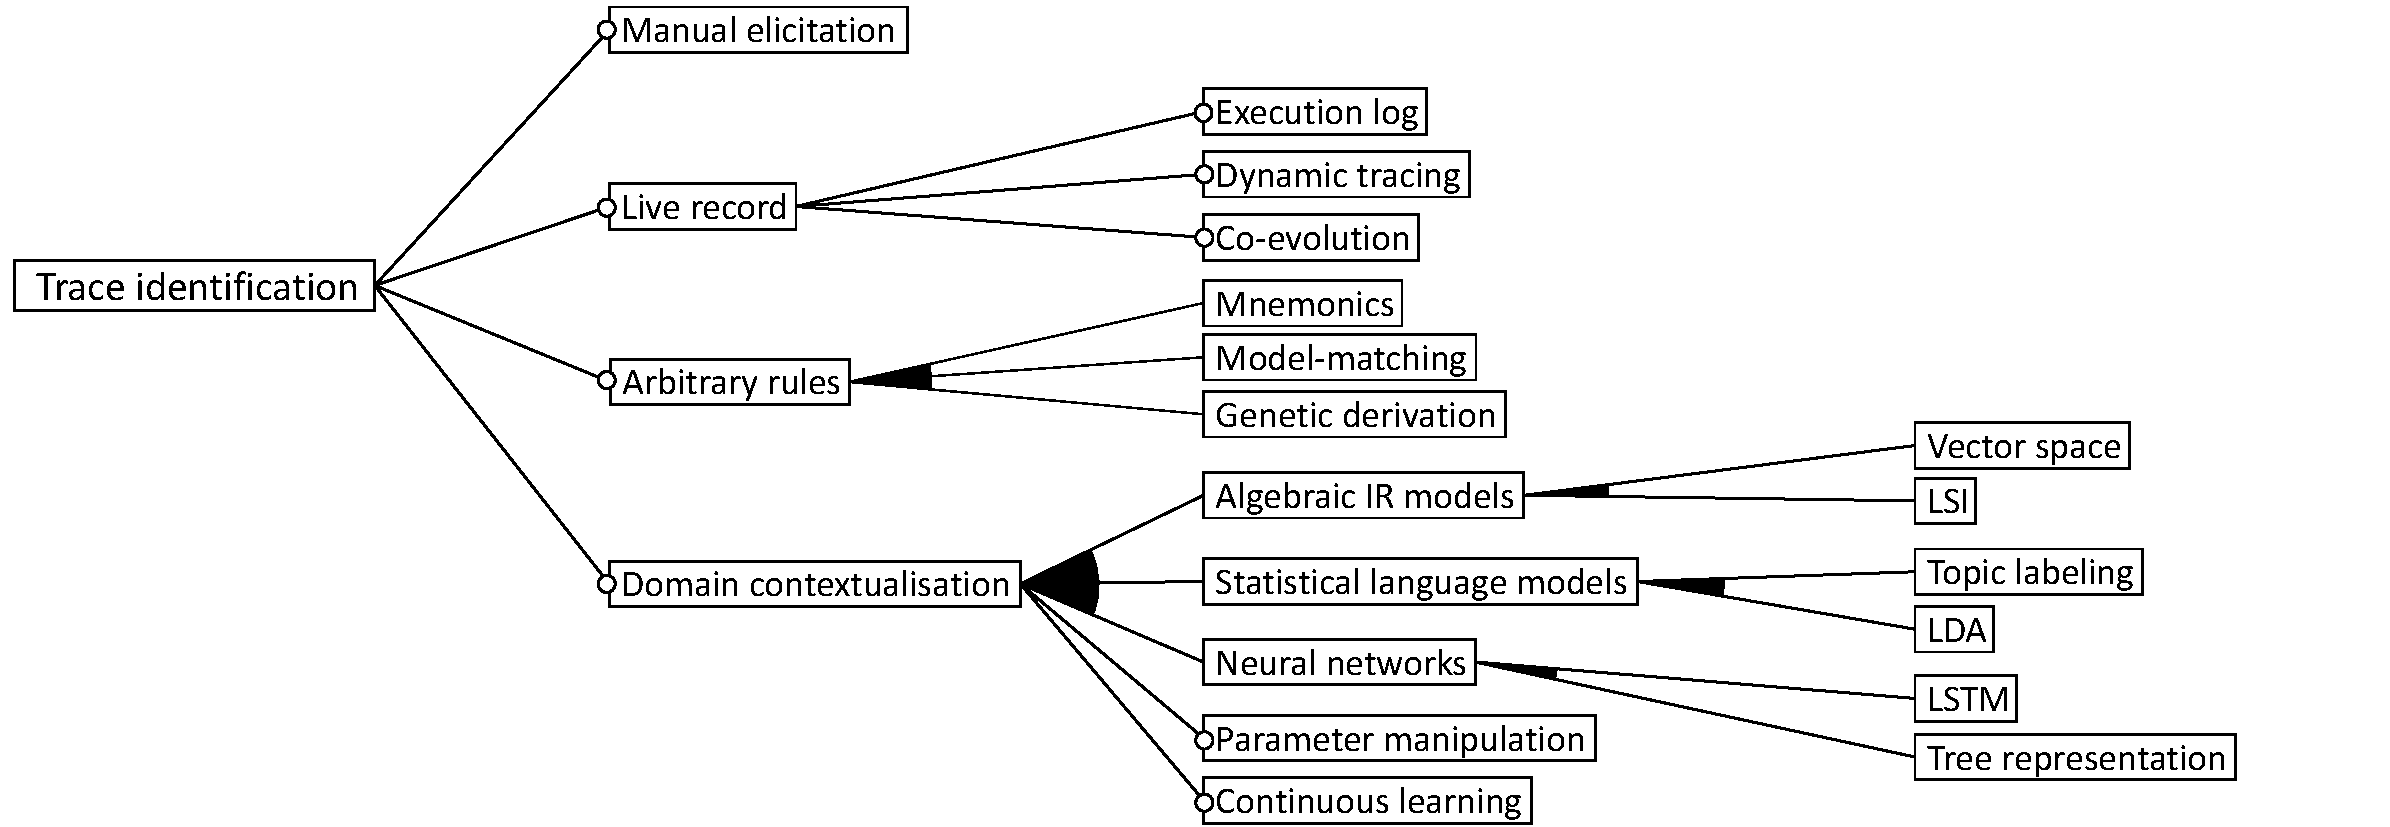
\includegraphics[width=.8\linewidth]{images/fm-identification}
	\caption{Features related to the identification of trace links}
	\label{fig:fm:identification}
\end{figure*}

%Many publications tackle the difficulty to automate the identification of trace links and introduce approaches based on the application of natural language processing techniques. 
\Fig{fig:fm:identification} shows the hierarchy of features related to the identification of traces with four main possible categories: 
the manual elicitation of traces, 
their live record during execution and evolution,
rule-based alternatives to assist the user with automation potential, 
and AI-augmented identification with domain contextualization.


\subsubsection{Manual elicitation} 
Manual elicitation makes possible to create traces in an \textit{ad hoc} manner. As an example, one of our industrial partner chose to hire a developer to elicit trace links necessary for a certification commitment. This was chosen rather than a (semi-)automated approach as they were not convinced the effort of augmenting an existing tool would pay off for that specific project. 

\subsubsection{Recording instrumentation} 
Teams can instrument the {live record} of traces during the execution and the evolution of software artefacts. This way traces recording the system changes are a side-effect of those same changes. There are initiatives to instrument existing languages such as ATL with rich log generation~\cite{Santiago_2013,la_Fosse_2018}, while others consider trace record an aspect that can be weaved with current existing languages~\cite{Pfeiffer_2014,Santiago_2013}. Ziegenhagen \textit{et al.} mix execution traces with metadatas~\cite{ziegenhagen2020-expanding-tracea-with-dynamic-tracing-data}, and use developer interaction records~\cite{ziegenhagen2019-developer-tool-interaction} to enrich existing traceability artefact.

Model transformations are considered the hearth and soul of software modeling and, consequently, numerous studies attempt to enrich trace generation during transformation execution~\cite{vara2014-traceability-in-MDD-MTransfo,Saada_2013,la_Fosse_2018}. This ubiquitous integration (see \Fig{fig:fm:management}, bottom branch) allows a semantically rich tracing of target and source artefacts~\cite{paige2011-traces-in-moel-driven-engineering}. Unfortunately, this option can only be applied when we are building the system, not when the system is already in place.

\subsubsection{Arbitrary rules} 
%Once a system is in place, the links that one might want to use (for locating features, increasing code understanding, and reducing perpetual maintenance effort) can be partly recovered automatically. Indeed, the knowledge that programmers process when writing the code is often captured by the mnemonics for identifiers~\cite{antoniol2002-tracing-code-documentation-links}. The analysis of these mnemonic means allows the constitution of linkage rules between software artefacts. The example of the similarity between Java classes file names and their respective binaries is obvious. 
Once a system is in place, teams can identify rules that help retrieve and maintain traceability relations~\cite{mader2008-rule-based-maintenance-post-requirements-traceability,spanoudakis2004-rule-based-generation-of-req-traceability-relations}.
Antoniol \textit{et al.} use the mnemonics for identifiers to establish trace identification rules~\cite{antoniol2002-tracing-code-documentation-links}.
At the model level, Grammel \textit{et al.} use a graph-based model matching technique to exploit metamodel matching techniques for the generation of trace links for arbitrary source and target models~\cite{grammel2012-model-matching-for-traceability-in-MDE}, and Saada \textit{et al.} recover  execution traces of model transformation using genetic algorithms~\cite{Saada_2013}.


\subsubsection{Domain contextualisation} 
Borillo \textit{et al.} published an article on the use of information retrieval techniques for linguistics applied to spatial software engineering~\cite{borillo1992-linguistic-engineering-to-spacial-SE}. This precursor work opened the box for AI-augmented traceability where machine learning algorithms help extract knowledge specific to the application domain. This is specially useful when the source (or target) of the trace link is an unstructured document or when such document is key to infer traces among other artefacts.

Researchers first extracted word vectors from natural language. Vectors intend to take account of the neighbouring words a term may relate to in the application domain~\cite{delucia2012-information-retrieval-for-traceability}. This effort made the identification of bonds between requirement specifications and other artefacts possible with a gradually improving precision. Since then, many other information retrieval techniques for natural language processing were applied with success~\cite{arunthavanathan2016-traceability-with-NLP}. Studies on domain contextualization are separated into three subgroups according to the type of tools used (algebraic information retrieval models, statistical language models, and neural networks).  For example, Florez \textit{et al.} derive fine grained requirement to source code links~\cite{florez2019-finegrained-req2code}, Rath \textit{et al.} complete missing links between commits and issues~\cite{rath2018-guo-augmenting-incomplete-traces}, Marcus \textit{et al.} identify links between documentation and source code~\cite{marcus2003-latent-semantic-indexing-for-traceability-LSI}. An interesting publication from Poshyvanyk \textit{et al.} shows that mixing expertise both in information retrieval techniques and engineering domains gives far better results than when taken separately~\cite{poshyvanyk2007}.

Today, domain contextualization by means of machine learning for topic modeling, word embedding, and more generally knowledge extraction from unorganized text documents is the most popular traceability feature~\cite{guo2017-semantically-enhanced-tracebility-deep-learning,wohlrab2020-traceability-organization-process-culture}. We found 22 approaches dedicated to this topic alone in our survey. 

Teams are also using genetic algorithms here, not to recover traces themselves but to cope with the variety of algorithms and parameters these approaches use~\cite{marcen2020-req2model-with-EA-ranking-train-system,panichella2013-genetic-programming-for-effective-topic-modeling}, and structural information to foster methodologies interweaving~\cite{panichella2013-using-structural-information-to-improve-IR-traceability}. Unfortunately, a common critique rose against these positive results. 
Too many teams compete with each others to accomplish a better precision and recall when there is no standard to the effective quantification of traces artefacts into such variables. Too few attempt at qualifying the overall relation between these measurement and the effective impact on software development~\cite{clelandhuang2014-traceability-trends-and-futurte-direction}. 

In that regard, Shin \textit{et al.} propose guidelines for benchmarking automated traceability techniques. Their evaluation (of 24 approaches) shows that methods of evaluation (when they are used appropriately) sometimes are not suitable to other application domains and that the variation in evaluation results across project is not investigated~\cite{shin2015-guidelines-benchmark-auto-traceability}. This corroborate Borg \textit{et al.} who, in a systematic literature mapping on information retrieval approaches to traceability, notice that there are no empirical evidence that any IR model outperforms another model consistently~\cite{borg2014-SmS-IR-for-traceability}. The ability to continuously improve the learning process is mentioned in the literature but we found no evidence of its application. 

\subsection{Trace management}
\label{sec:fm:toolsupport}
\begin{figure*}[h]
	\centering
	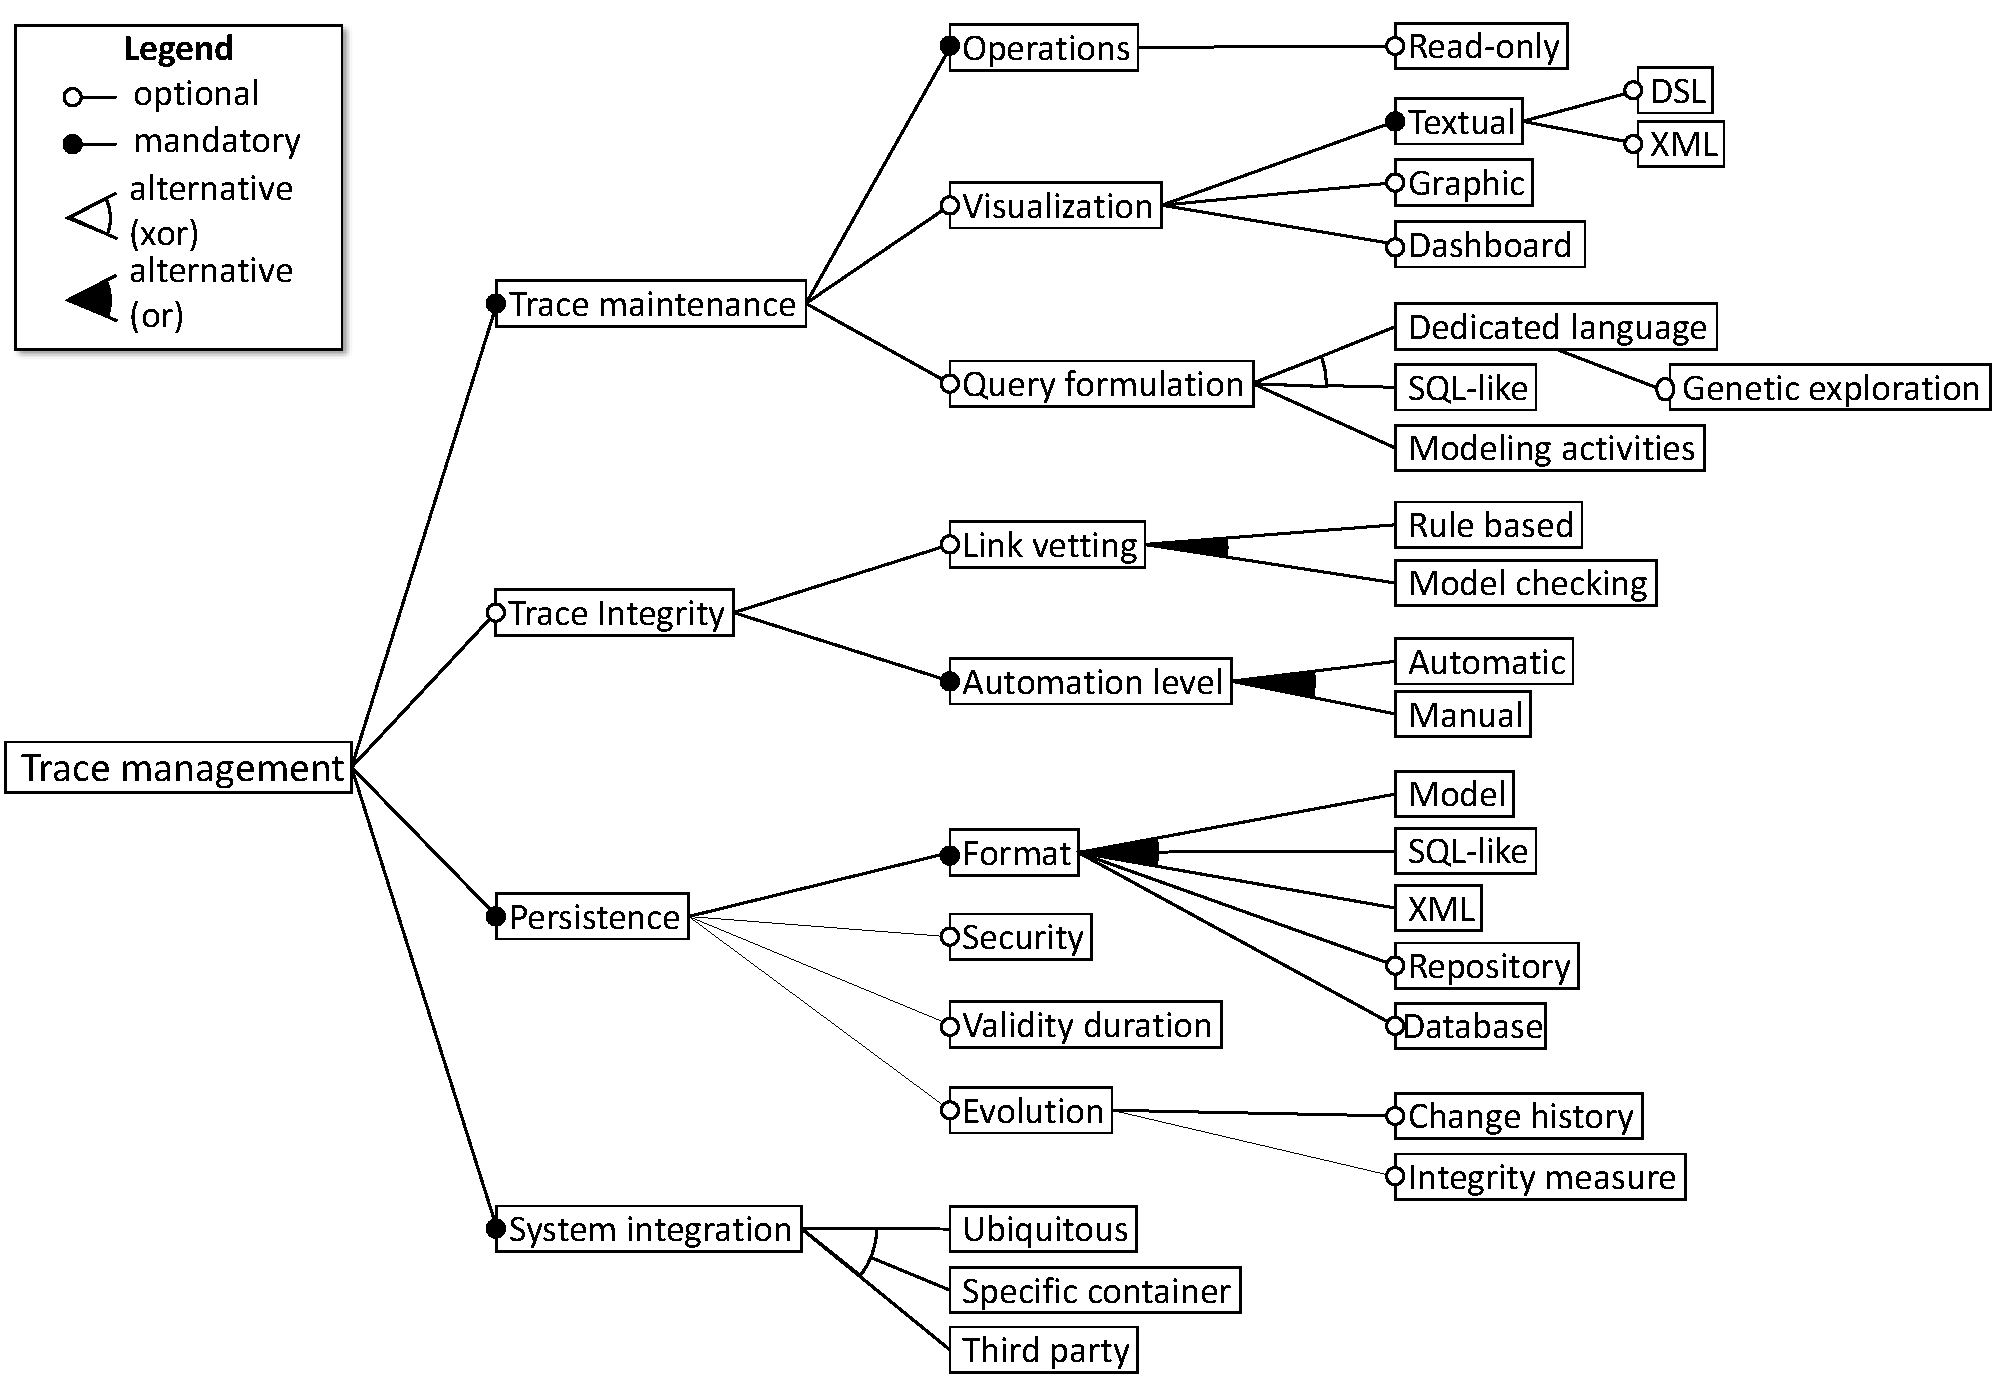
\includegraphics[width=.8\linewidth]{images/fm-toolsupport}
	\caption{Tool support for traceability management.}
	\label{fig:fm:management}
\end{figure*}

\Fig{fig:fm:management} shows the hierarchy of features related to the management of trace artefacts. We distinguish between the actual maintenance of trace artefacts, the evaluation of their integrity, the means of persistence, and the level of integration in running software systems.

\subsubsection{Trace Maintenance} 
Trace links may be affected by changes on the artefacts they are linking to (directly or transitively) and therefore can easily become obsolete. This gradual decay must be seriously taken into account to avoid having to re-elicit traces every time they need to be analyzed. A manual maintenance is not always impossible but not typically feasible in practice due to the amount of information such inspections would involve. % This motivates a serious consideration of automated ways to retrieve and then visualise traces. 
%The vast amount of potential trace links traceability approaches have to handle motivate a serious consideration of automated ways to visualise and retrieve them. 
Co-evolution techniques~\cite{mader2008-rule-based-maintenance-post-requirements-traceability,drivalos2010-state-based-traceability,rahimi2019-Evolving-trace-req2source} attempt to tackle the burden to maintain trace links up-to-date~\cite{seibel2010-dynamic-hierarchical-models-comprehensive-traceability,Bunder_2017_query-for-quality}. 

Beyond being able to manipulate traces, we also need to offer proper ways to visualize and inspect them~\cite{fittkau2013-explorviz-Trace-Visualization}. The use of graphical representations stimulate human perception and the integration of such technique in traceability frameworks is a useful feature to augment user awareness~\cite{heisig2019-generic-traceability-metamodel-end-to-end-capra}.
In parallel, allowing a rich formulation of queries to assist the exploration of existing traces will help to reduce the amount of information users need to navigate through~\cite{Bunder_2017_query-for-quality}.
More precisely, structured text, in the form of metamodel instances or XML sheets allows query-based mining of trace datasets~\cite{dietrich2013-learning-efective-query-transformation-for-enhanced-req-trace-retrieval}. Interaction wise, hyper-text links is a \textit{de facto} standard to browse trace links. Indeed, following links through successive clicks has become almost natural.  Querying depends on the type of representation of traceability artefacts. SQL-like languages benefit from a long history of information mining while dedicated languages offers better legibility. Genetic programming has also permitted the automation of query formulation~\cite{perez2020-genetic-query-reformulation-for-feature-location}. 

%All in all, assisting efficiently end-users in the retrieval, visualization and analysis of traces is not easily granted. Yet, studies on the topic remain scarce in comparison to other concerns. There is still great space for improvement and calls for more work in that direction are redundant through literature studies~\cite{Gotel2012,antoniol2017-traceability-grand-challenges}.

\subsubsection{Trace Integrity} 
To cope with the decay and volatility mentioned above, we need a way to determine the integrity of existing traces. Work on these questions, although called out loudly by literature studies, is scarce in practice~\cite{winkler2010-survey-traceability-and-MDE,antoniol2017-traceability-grand-challenges}. The first option is given with manual annotation or vetting of trace links to inform about their level of reliability. Annotations allow a qualitative and quantitative evaluation~\cite{Buchmann_2015}. This is the case for back-propagation of verification and validation results between design and requirements~\cite{Hegedus_2010}.  

Some approaches enable the definition of invariant rules while manipulating traces or their targets~\cite{Bunder_2017_query-for-quality}. If the invariant is violated, an exception for that trace is automatically generated. For example, we could define a rule that is violated when a change occurs in an artefact targeted by a trace if the corresponding link was identified more than two versions prior to the current version. 

\subsubsection{Trace persistence} 
\ugh{Security?}

Many different storage alternatives exist for traceability artefacts.
An option is to use SQL-like grammar to store and retrieve traces with the power of database tooling, or to use XML documents to represent trace matrix in a transformable format. The industry uses a lot of informal format and link representations often remain implemented in spreadsheets, text files, databases or requirement management tools. These links deteriorate quickly during a project as time pressured team members fail to update them. 
Researchers aiming at a generalizable approach favour model-based representations able to express specifically defined concepts related to traceability (often in a specific domain of application). The burden of maintaining traces coherent is eased in model-based solutions~\cite{clelandhuang2007bestPracticeForAutomatedTraceability}. Elamin \textit{et al.} propose to implement traceability artefact in graph based databases to improve software quality~\cite{elamin2018-repositories-as-graph-databases}.

Another concern lies in the recording of trace evolution. The trace creation should be recorded, with the successive changes that affect it, for evolution analysis. Integrity measures respective to evolution events (\textit{e.g.,} creation, modification...) should be recorded as well to evaluate their evolution during a period of time. Rahimi \textit{et al.} ensure the co-evolution of artefacts and traces~\cite{rahimi2019-Evolving-trace-req2source} using a set of heuristics coupled with refactoring detection and information retrieval to detect changes scenario between contiguous versions of software systems.

\subsubsection{System integration} 
Like most of the MDe approaches, Helming \textit{et al.} use of the same modeling language for both traceability and system artefacts to track changes~\cite{helming2009-traceability-change-awareness}. The conjunct use of EMF and a dedicated traceability metamodel (both written in Ecore) facilitates the integration of traceability features including graphical versions to stimulate human perception and standard analysis of traces in the native (Ecore) environment of the traced system. 

Galvao \textit{et al.} in their seminal work on traceability and MDE call for more loosely coupled traceability support that can integrate external relationship with independent representations (in another, ideally common language)~\cite{galvao2007-survey-traceability-in-MDE} as also elaborated by Azevedo \textit{et al.}~\cite{azevedo2019-traceability-metamodel-and-reference-model}. 



